\documentclass[11pt,a4paper]{article}
\usepackage[utf8]{inputenc}
\usepackage{amsmath,amssymb}
\usepackage{graphicx}
\usepackage{subcaption}
\usepackage{hyperref}
\usepackage{geometry}
\usepackage{xcolor}

\geometry{margin=1in}
\graphicspath{{../../figures/}}

\title{The Doubt Variable as Anti-Synchronization Filter:\\Topological Diversity Boundaries and Their Adaptive Resolution}
\author{Mem4ristor Project Consortium}
\date{\today}

\begin{document}

\maketitle

\begin{abstract}
Coupled oscillator networks often collapse into homogeneous states when simulated on dense scale-free topologies. In the extended FitzHugh-Nagumo model equipped with a metacognitive ``doubt'' variable ($u$), this structural trap is absolute for Barab\'asi-Albert networks of parameter $m \geq 5$---a \emph{Topological Dead Zone} that no linear coupling normalization can break. We demonstrate that the doubt variable functions primarily as an active anti-synchronization filter rather than an optimal decoder of topological surprise. Ablating the local disagreement signal driving $u$ and replacing it with pure noise or its static temporal mean preserves network diversity (absolute $\Delta H_{\mathrm{cog}} = 0.0027$ bits, $0.115\%$ of maximum entropy $\log_2 5 = 2.32$ bits), whereas completely freezing $u$ induces a $985\%$ surge in pairwise synchrony. Furthermore, the characteristic timescale of doubt, $\tau_u$, serves as a master bifurcation parameter, with a critical transition around $\tau_u \approx 10$ separating regimes of frozen frustration and breathing chimeras. Through extensive numerical simulations and finite-size scaling ($N$ up to $1600$), we map the phase boundary defined by the algebraic connectivity $\lambda_2$ and reveal that stochastic resonance via uniform thermal noise provides a topology-dependent escape, which is robust only for $\lambda_2 < 2.5$.
\end{abstract}

\section{Introduction}
\label{sec:intro}
Scale-free topologies represent the structural foundation of biological and artificial neural networks. However, in models of coupled oscillators, the presence of densely connected hubs inherently biases the system toward global synchronization, erasing the very cognitive diversity these networks are designed to support. This phenomenon, formalized as the \textit{Topological Dead Zone}, describes the inability of conventional coupling mechanisms to sustain distinct attractor states when the network's algebraic connectivity exceeds a critical threshold ($\lambda_2 \approx 2.5$).

While earlier investigations (Paper 1) established that doubt-modulated coupling can sustain diversity on regular lattices and sparse scale-free networks, denser topologies ($m \geq 5$) remain impenetrable traps. This paper delineates the strict topological boundary of the doubt mechanism and redefines the role of the doubt variable ($u$) itself: not as a decoder of structural surprise, but as an essential, robust anti-synchronization filter.

\section{The $u$ Variable: Mechanism and Ablation}
\label{sec:mechanism}
To isolate the causal role of the metacognitive doubt variable $u$, we performed targeted ablations of the local disagreement signal ($\sigma_{\mathrm{social}}$) that drives it. If $u$ acts as a precise decoder of topological structural information, replacing its driving signal with noise should collapse the network's diversity.

Our results refute this hypothesis. Replacing $\sigma_{\mathrm{social}}$ with a pure Gaussian noise sequence matched to its root-mean-square amplitude (\textsc{SS\_NOISE}) or its static temporal mean (\textsc{SS\_STATIC}) produces cognitive entropy and pairwise synchrony indistinguishable from the full model (absolute $\Delta H_{\mathrm{cog}} = 0.0027$ bits ($0.115\%$ of maximum entropy $\log_2 5 = 2.32$ bits); $\Delta\mathrm{sync} < 24\%$ relative to the FULL baseline). The network is profoundly insensitive to the informational content of the disagreement signal.

However, the variable $u$ itself is absolutely necessary. Freezing $u$ entirely (\textsc{FROZEN\_U}) collapses the network into a hyper-synchronized regime. Pairwise synchrony surges by $+985\%$, and the system adopts a globally coherent limit-cycle oscillation. This establishes $u$ as an active anti-synchronization filter: its continuous modulation of coupling polarity actively decorrelates neighboring nodes, maintaining spatial mutual information strictly below that of ablated models across all distances. The doubt variable does not decode the topology; it constantly perturbs it to prevent consensus.

\begin{figure}[htbp]
  \centering
  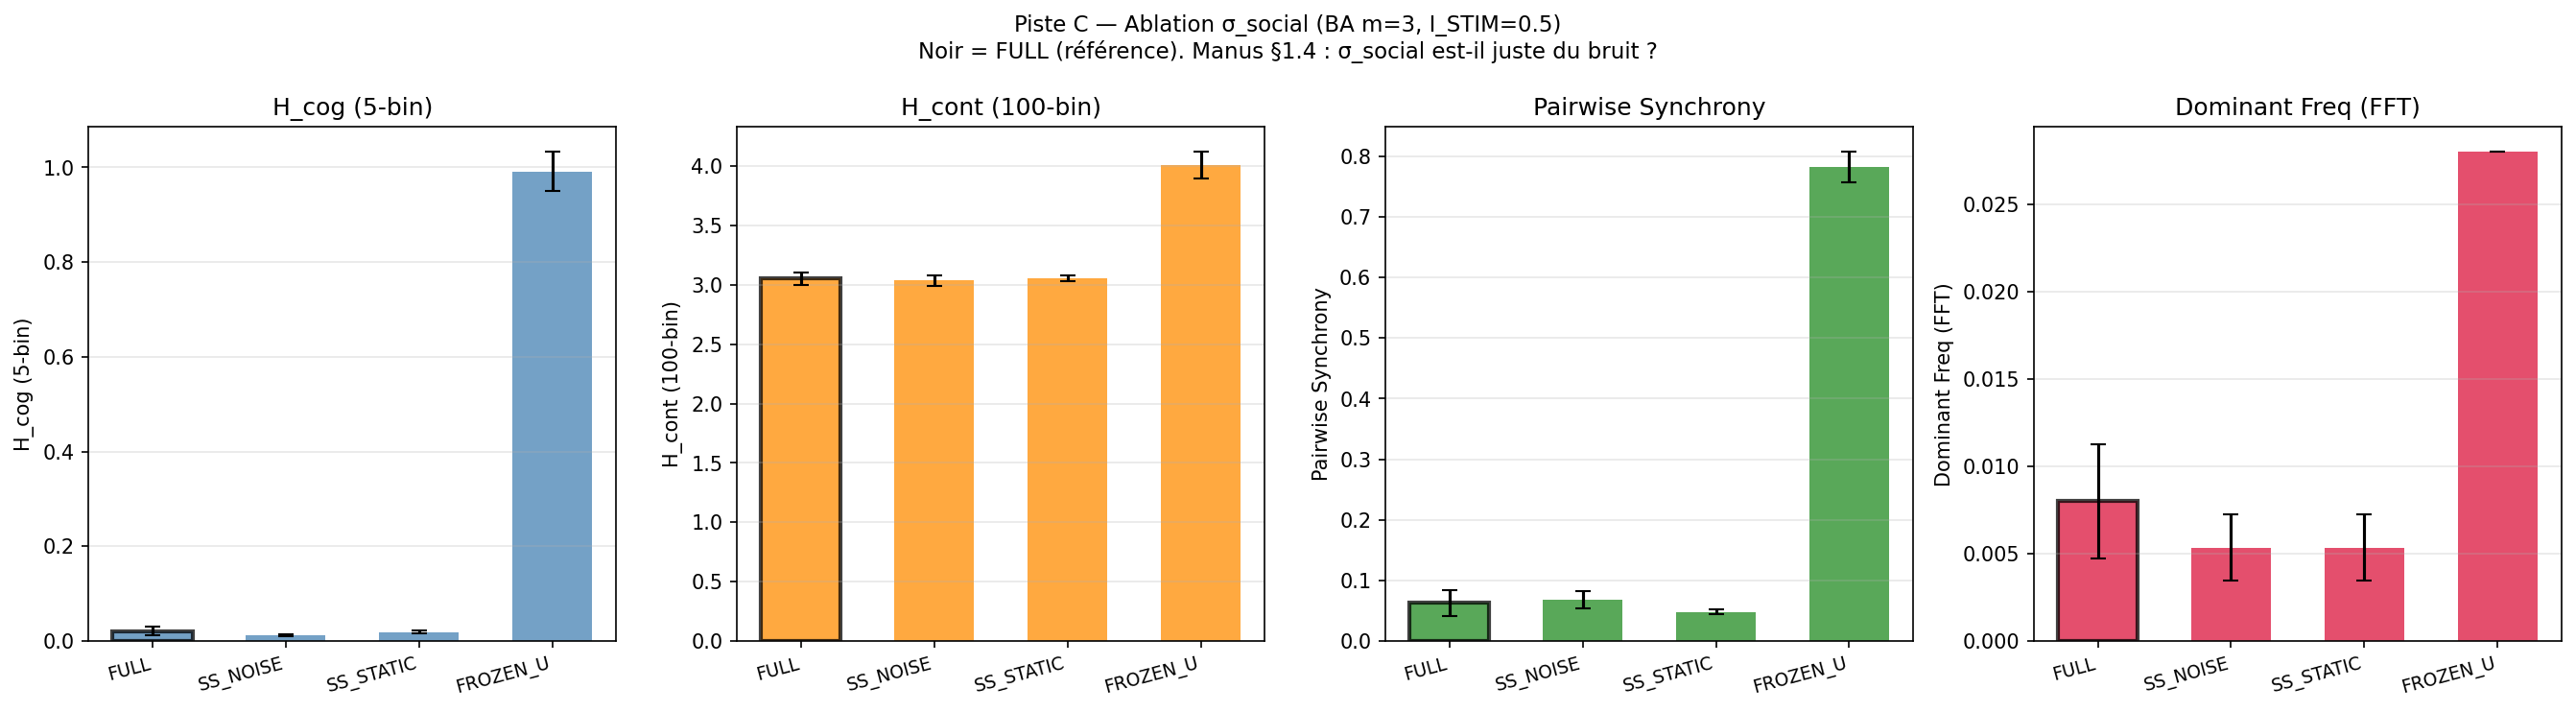
\includegraphics[width=0.88\linewidth]{p2_sigma_social_ablation.png}
  \caption{Ablation of the $\sigma_{\mathrm{social}}$ signal driving the doubt variable $u$, on a Barab\'asi-Albert network ($m=3$, $N=100$, $I_{\mathrm{stim}}=0.5$, mean over 5 seeds). Four conditions are shown: \textsc{FULL} (reference), \textsc{SS\_NOISE} ($\sigma_{\mathrm{social}}$ replaced by amplitude-matched Gaussian noise), \textsc{SS\_STATIC} ($\sigma_{\mathrm{social}}$ frozen at its temporal warmup mean), and \textsc{FROZEN\_U} (adaptive epsilon set to zero, $u$ fixed). Left: cognitive entropy $H_{\mathrm{cog}}$. Right: mean pairwise synchrony. \textsc{SS\_NOISE} and \textsc{SS\_STATIC} are indistinguishable from \textsc{FULL}, while \textsc{FROZEN\_U} triggers a $+985\%$ synchrony surge ($n=5$ seeds).}
  \label{fig:ablation}
\end{figure}

\begin{figure}[htbp]
  \centering
  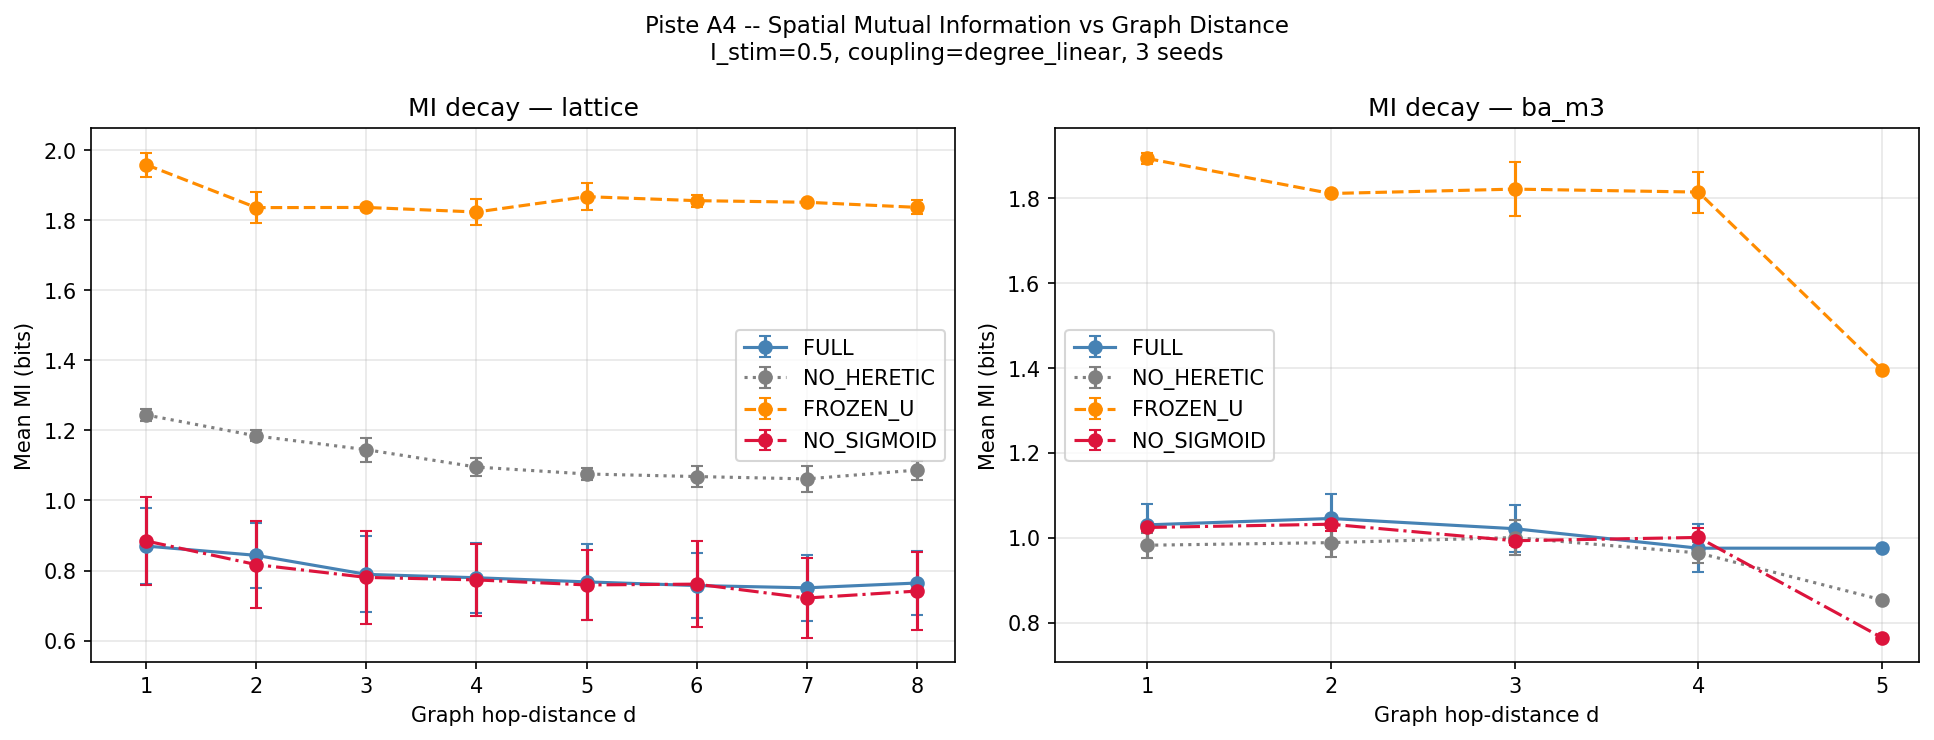
\includegraphics[width=0.88\linewidth]{p2_spatial_mutual_information.png}
  \caption{Spatial mutual information $I(v_i; v_j)$ as a function of topological distance (hop count) on the BA $m=3$ network, for the four ablation conditions. The \textsc{FROZEN\_U} condition maintains high mutual information at all distances, while the three active-$u$ conditions (\textsc{FULL}, \textsc{SS\_NOISE}, \textsc{SS\_STATIC}) are mutually indistinguishable and exhibit rapid decorrelation with distance. This confirms that $u$ operates as a topological decorrelator regardless of its driving signal.}
  \label{fig:spatial_mi}
\end{figure}

\section{$\tau_u$ as a Master Control Parameter}
\label{sec:bifurcation}
The characteristic timescale of the doubt variable, $\tau_u$, determines the network's capacity to adapt to local frustration. A systematic sweep of $\tau_u$ under forced conditions ($I_{\mathrm{stim}}=0.5$) reveals a sharp bifurcation. For fast doubt dynamics ($\tau_u < 10$), the system is trapped in a regime of frozen frustration, where rapid coupling polarity flips lock the network into a pseudo-consensus state ($H_{\mathrm{cog}} \approx 0.02$). For slower dynamics ($\tau_u > 50$), the network transitions into a ``breathing chimera'' regime ($H_{\mathrm{cog}} \approx 0.38$), where dynamic clusters form and dissolve.

\begin{figure}[htbp]
  \centering
  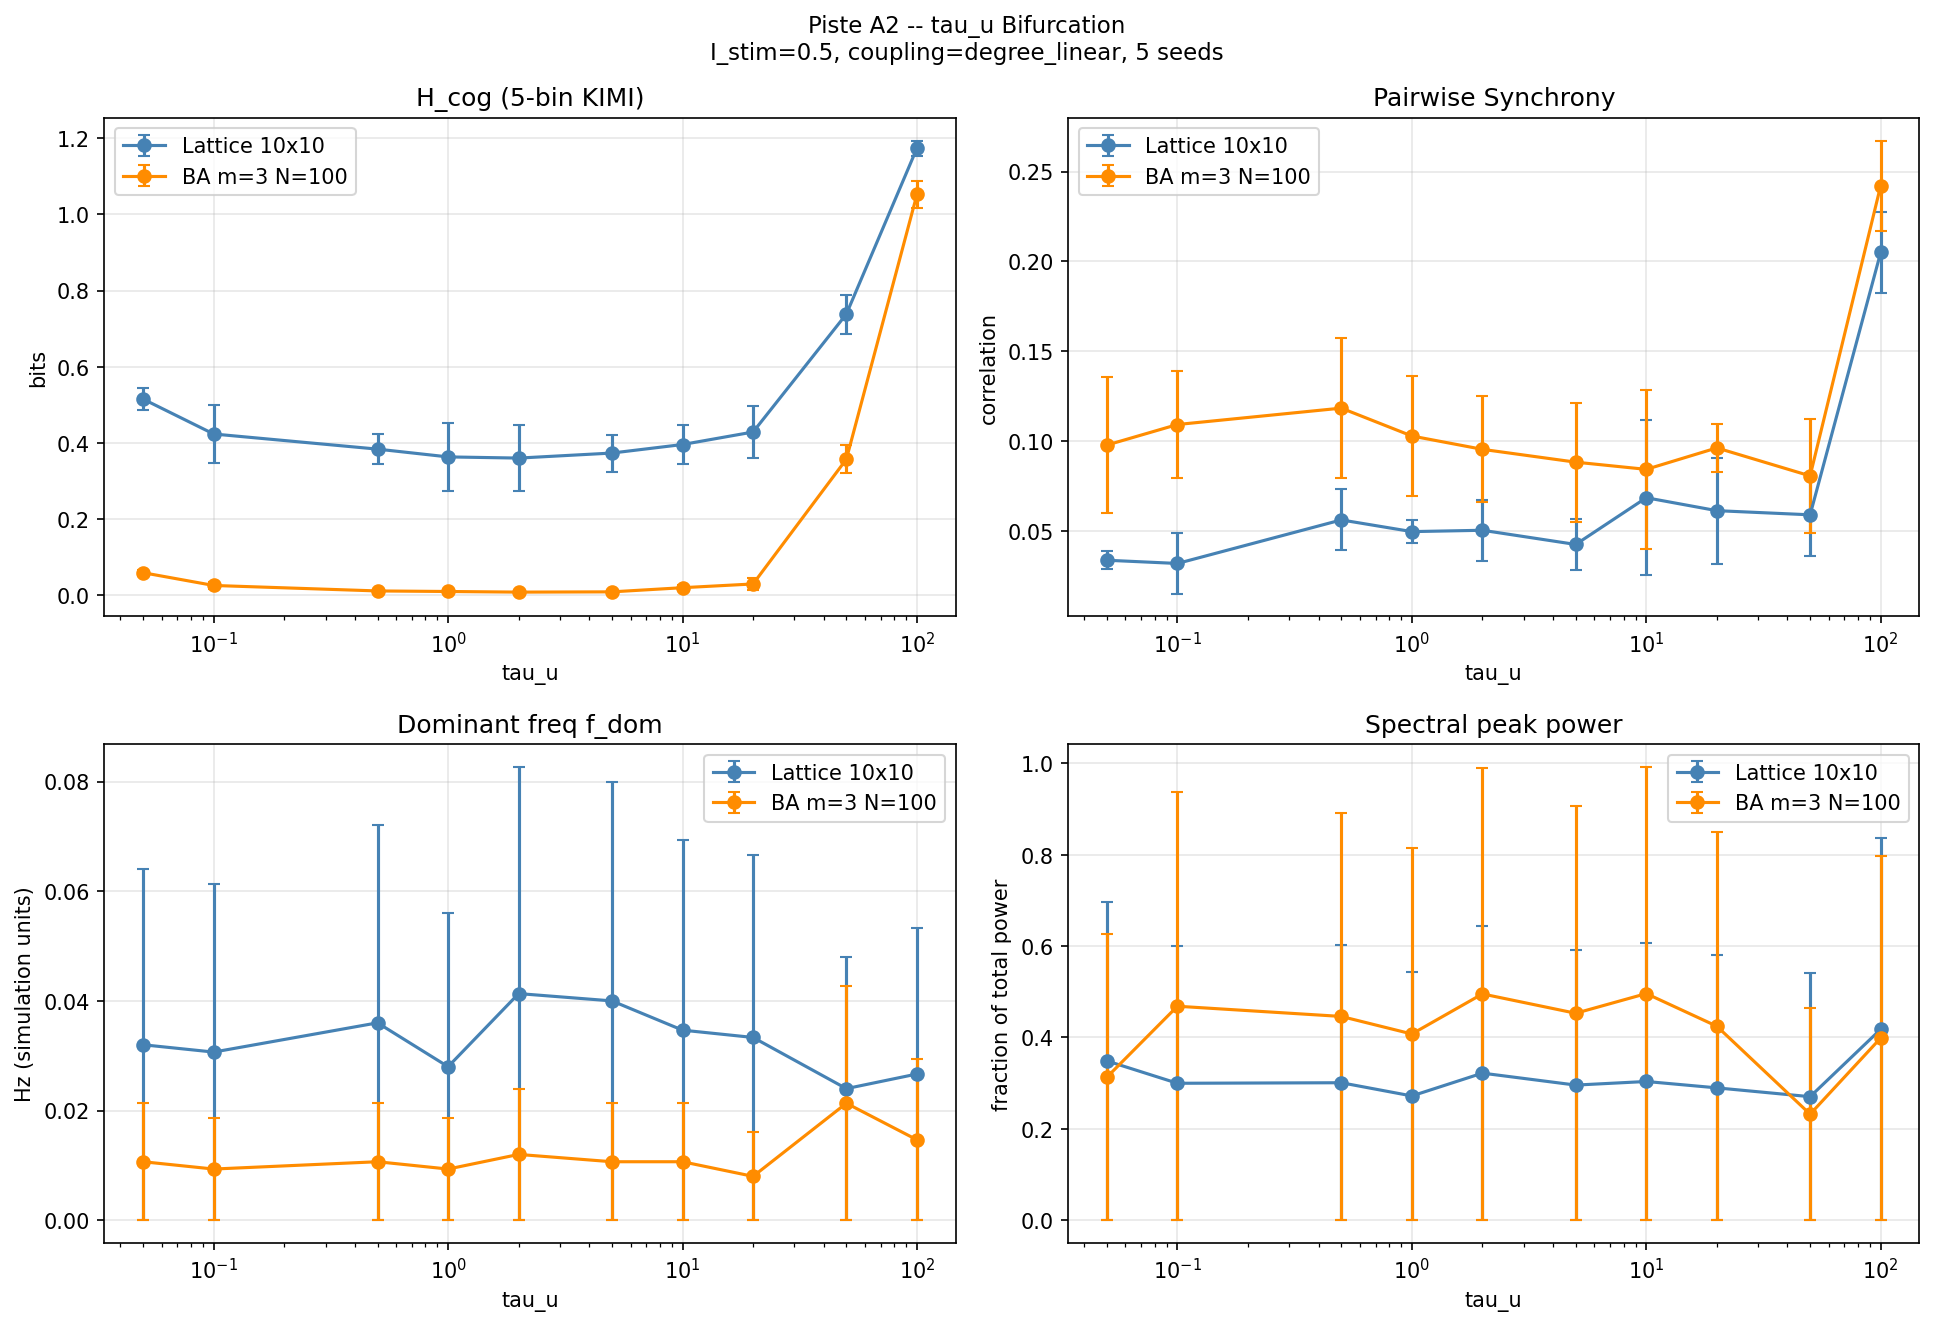
\includegraphics[width=0.88\linewidth]{p2_tau_u_bifurcation.png}
  \caption{Bifurcation in cognitive entropy $H_{\mathrm{cog}}$ and mean pairwise synchrony as a function of the doubt timescale $\tau_u$, under forced stimulation ($I_{\mathrm{stim}}=0.5$). Results are shown for the regular lattice ($10{\times}10$) and BA $m=3$ ($N=100$), averaged over 5 seeds. A critical transition near $\tau_u \approx 10$ separates frozen-frustration ($H_{\mathrm{cog}} \approx 0.02$) and breathing-chimera ($H_{\mathrm{cog}} \approx 0.38$) regimes.}
  \label{fig:tau_bifurcation}
\end{figure}

Strikingly, this bifurcation persists even in the purely endogenous regime ($I_{\mathrm{stim}}=0.0$), where structural heretics are mathematically inactive. In the absence of external forcing, the system lacks the symmetry-breaking required to occupy distinct physiological states (yielding a binning artifact where $H_{\mathrm{cog}} \approx 0$), yet the continuous sub-threshold entropy $H_{\mathrm{cont}}$ clearly traces the identical bifurcation: peaking at $\tau_u = 5$ before collapsing as $\tau_u \to 50$. This confirms that $\tau_u$ intrinsically governs the coherence of the network, independently of stimulus.

\begin{figure}[htbp]
  \centering
  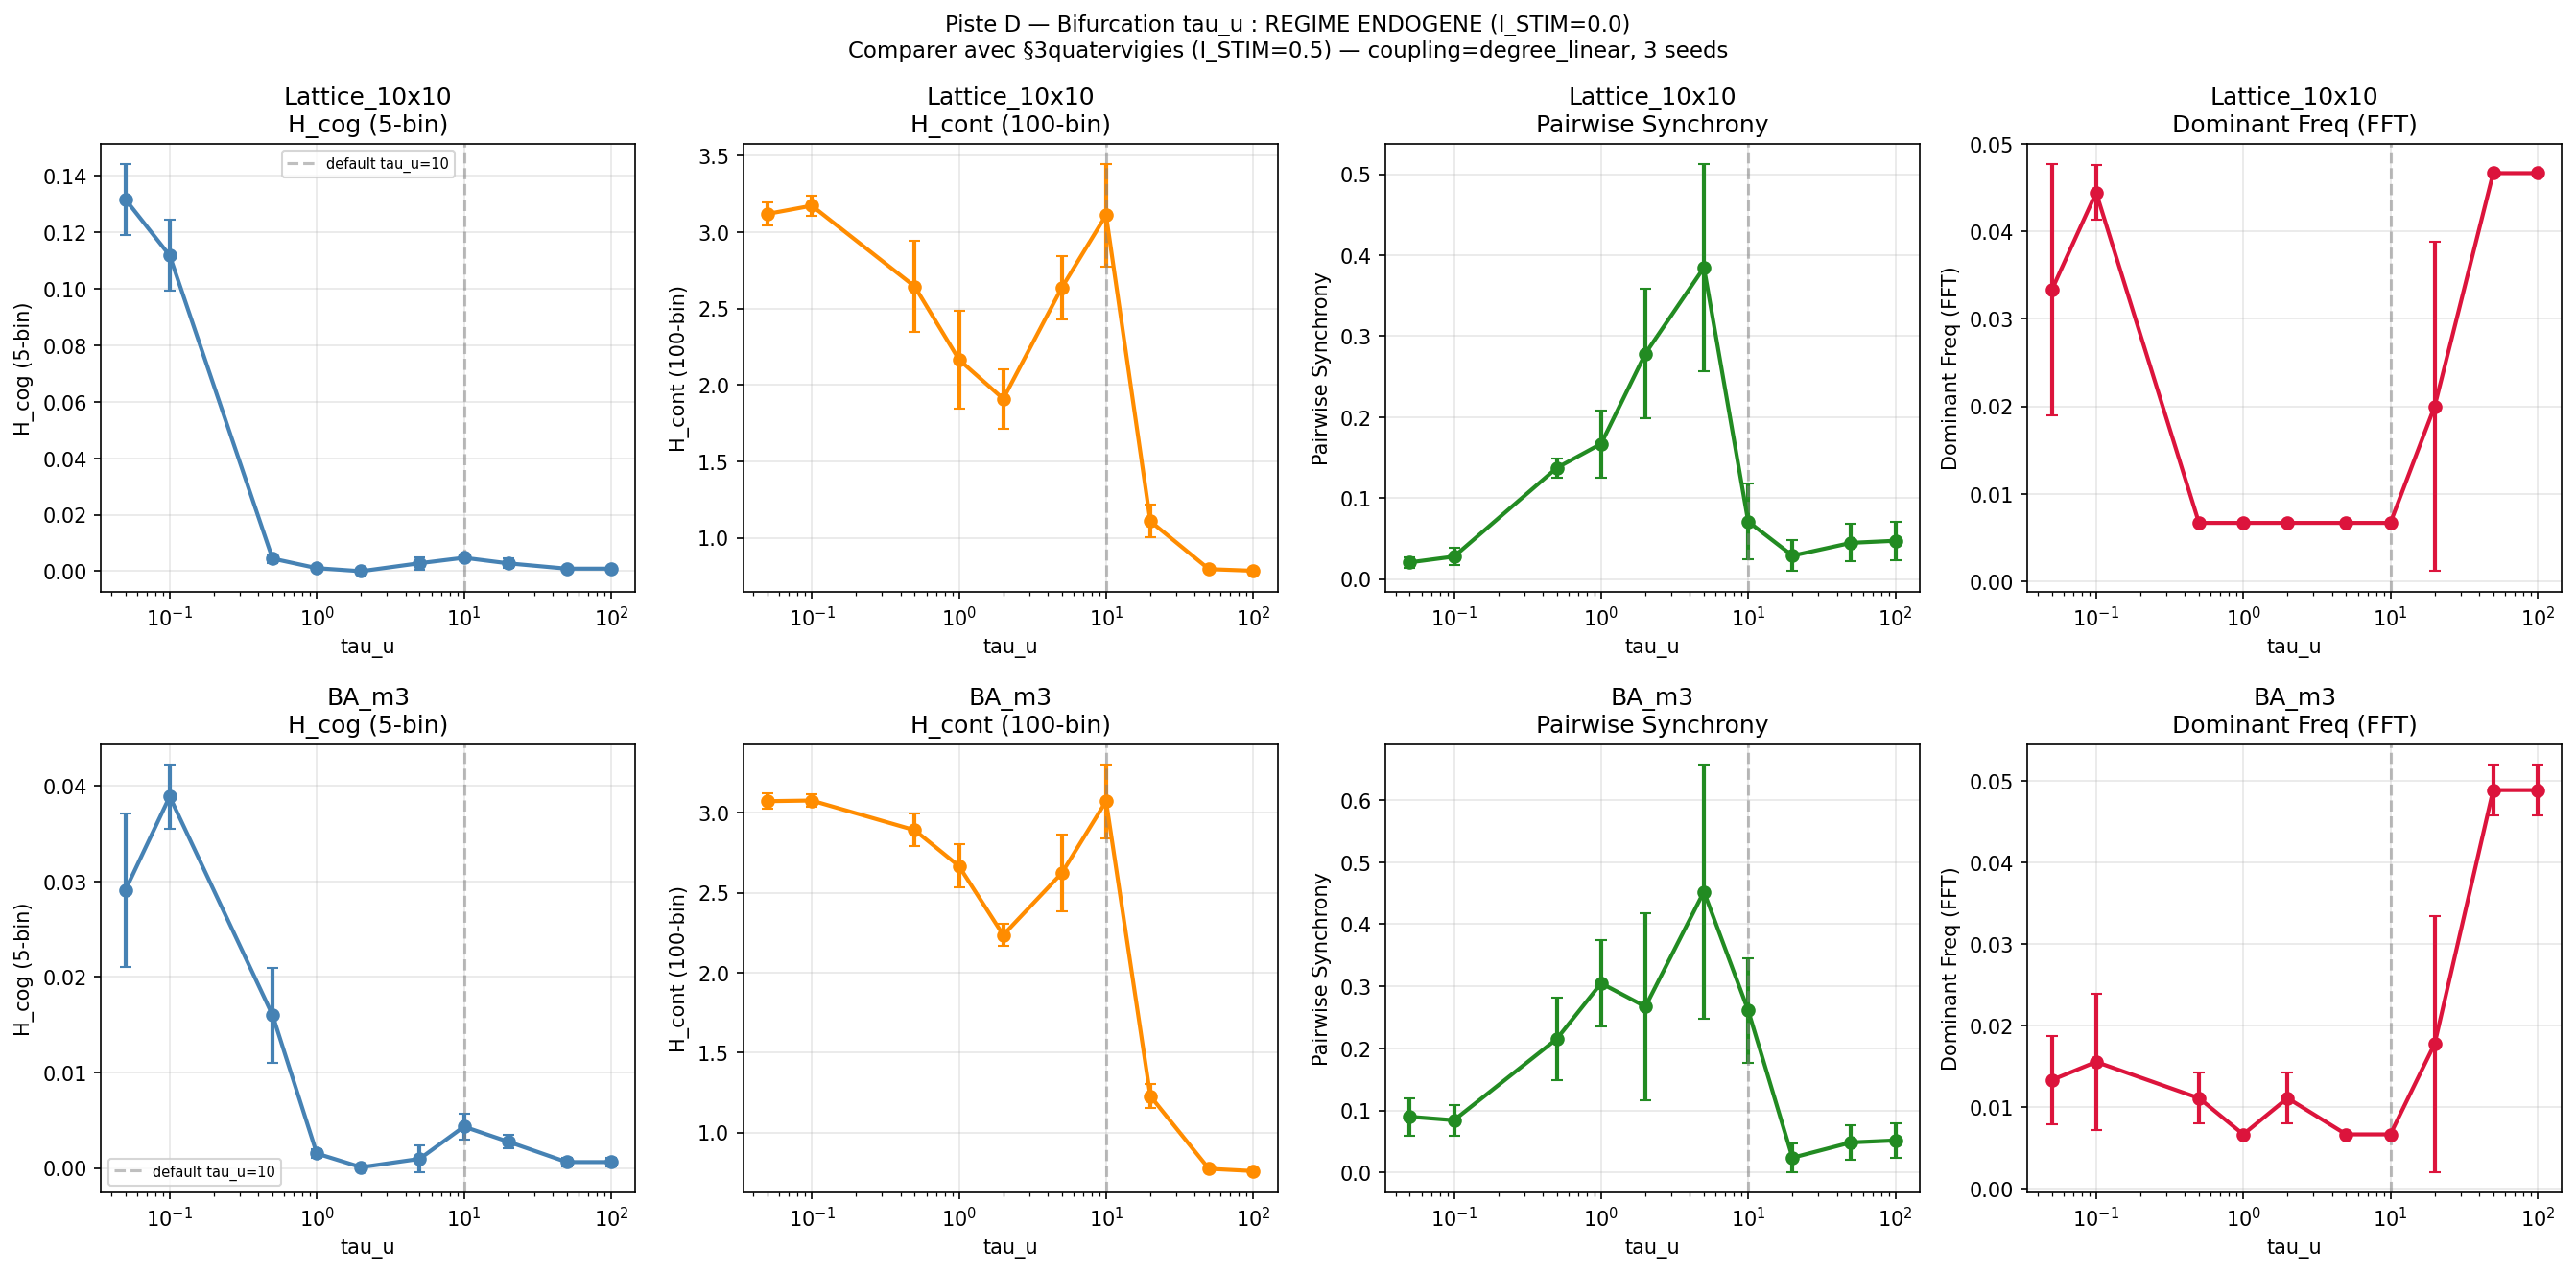
\includegraphics[width=0.88\linewidth]{p2_tau_u_bifurcation_endogenous.png}
  \caption{Endogenous $\tau_u$ bifurcation ($I_{\mathrm{stim}}=0.0$). Discrete cognitive entropy $H_{\mathrm{cog}}$ (solid) remains near zero due to the binning artifact (all nodes near the resting fixed point $v^* \approx -1.29$), but the continuous sub-threshold entropy $H_{\mathrm{cont}}$ (dashed) recovers the same bifurcation shape as in the forced regime, confirming that $\tau_u$ governs coherence intrinsically.}
  \label{fig:tau_endogenous}
\end{figure}

\section{Topological Phase Boundary}
\label{sec:phase_boundary}
The topological dead zone observed on dense Barab\'asi-Albert networks ($m \geq 5$) resists all linear coupling normalization schemes, including degree-linear and spectral normalization (eigenvector centrality). The controlling parameter is not the local degree heterogeneity, but the global path redundancy, parameterized by the algebraic connectivity $\lambda_2$.

A structural analysis of 12 distinct topologies reveals that $\lambda_2$ is a near-perfect predictor of the dead zone regime ($r = +0.901, p < 10^{-4}$), vastly outperforming edge betweenness centrality ($r = -0.604$). Finite-size scaling analyses spanning $N=100$ to $N=1600$ demonstrate that $\lambda_2$ is scale-invariant for a given $m$, and that the critical threshold $\lambda_{2,\mathrm{crit}} \approx 2.5$ represents a strict structural boundary.

\begin{figure}[htbp]
  \centering
  \begin{subfigure}[b]{0.48\linewidth}
    \centering
    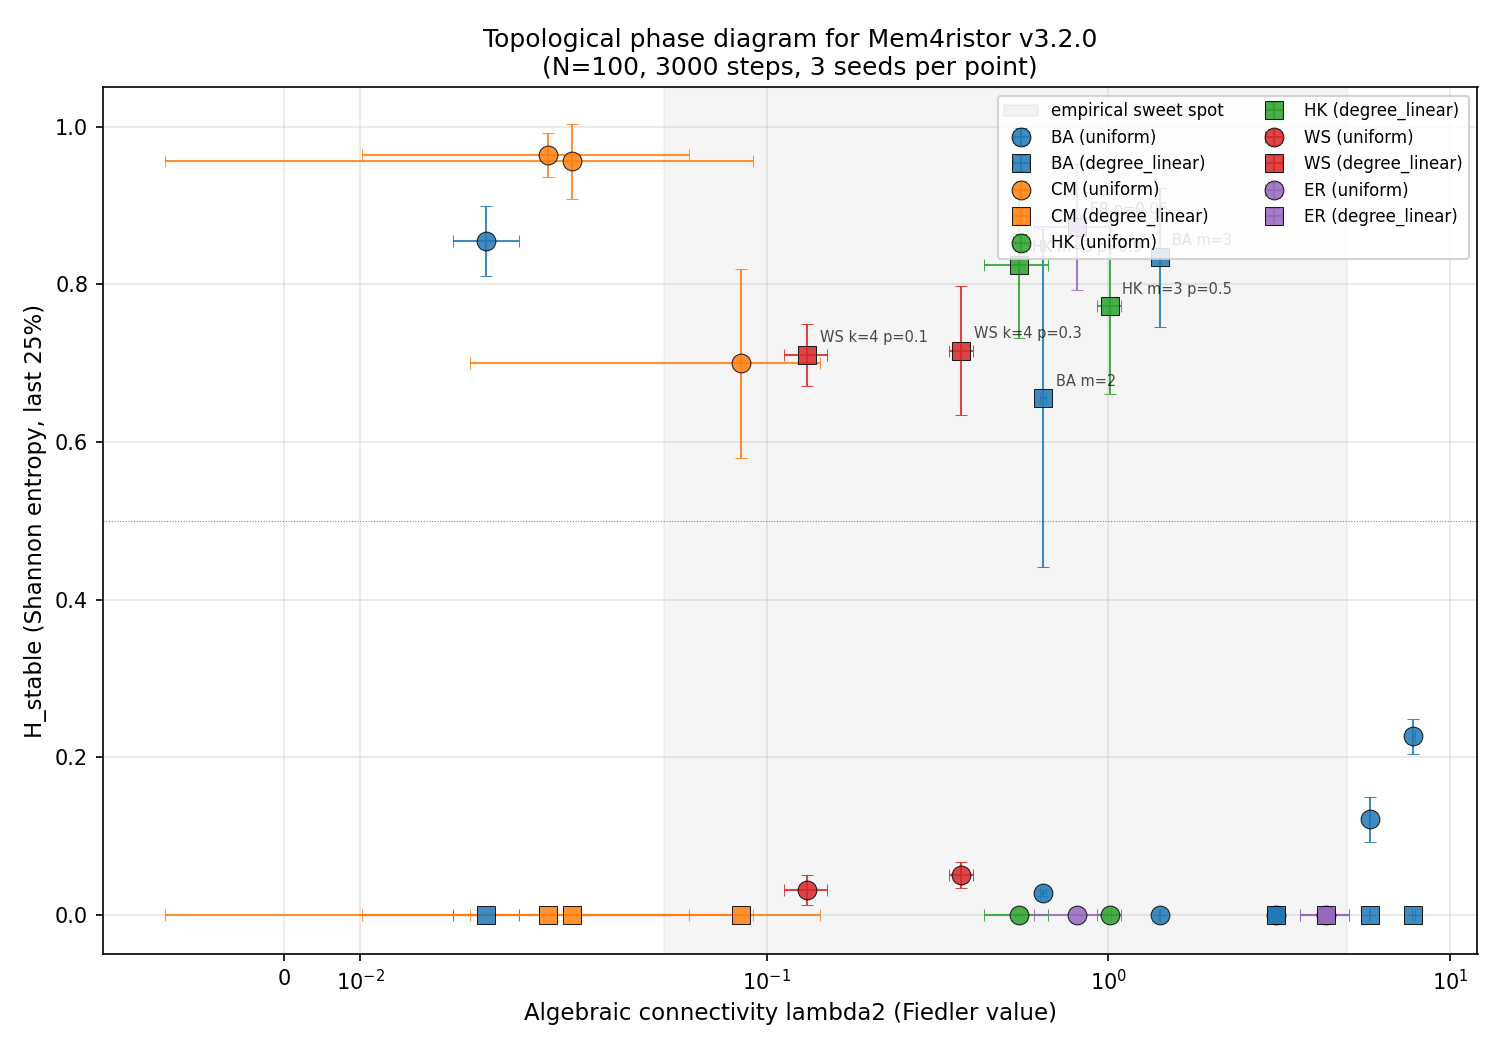
\includegraphics[width=\linewidth]{fiedler_phase_diagram.png}
    \caption{Phase diagram: cognitive entropy vs.\ $\lambda_2$ across 12 topologies. A dead zone is evident above $\lambda_{2,\mathrm{crit}} \approx 2.5$ (dashed vertical line); Pearson $r = +0.901$, $p < 10^{-4}$.}
    \label{fig:fiedler}
  \end{subfigure}
  \hfill
  \begin{subfigure}[b]{0.48\linewidth}
    \centering
    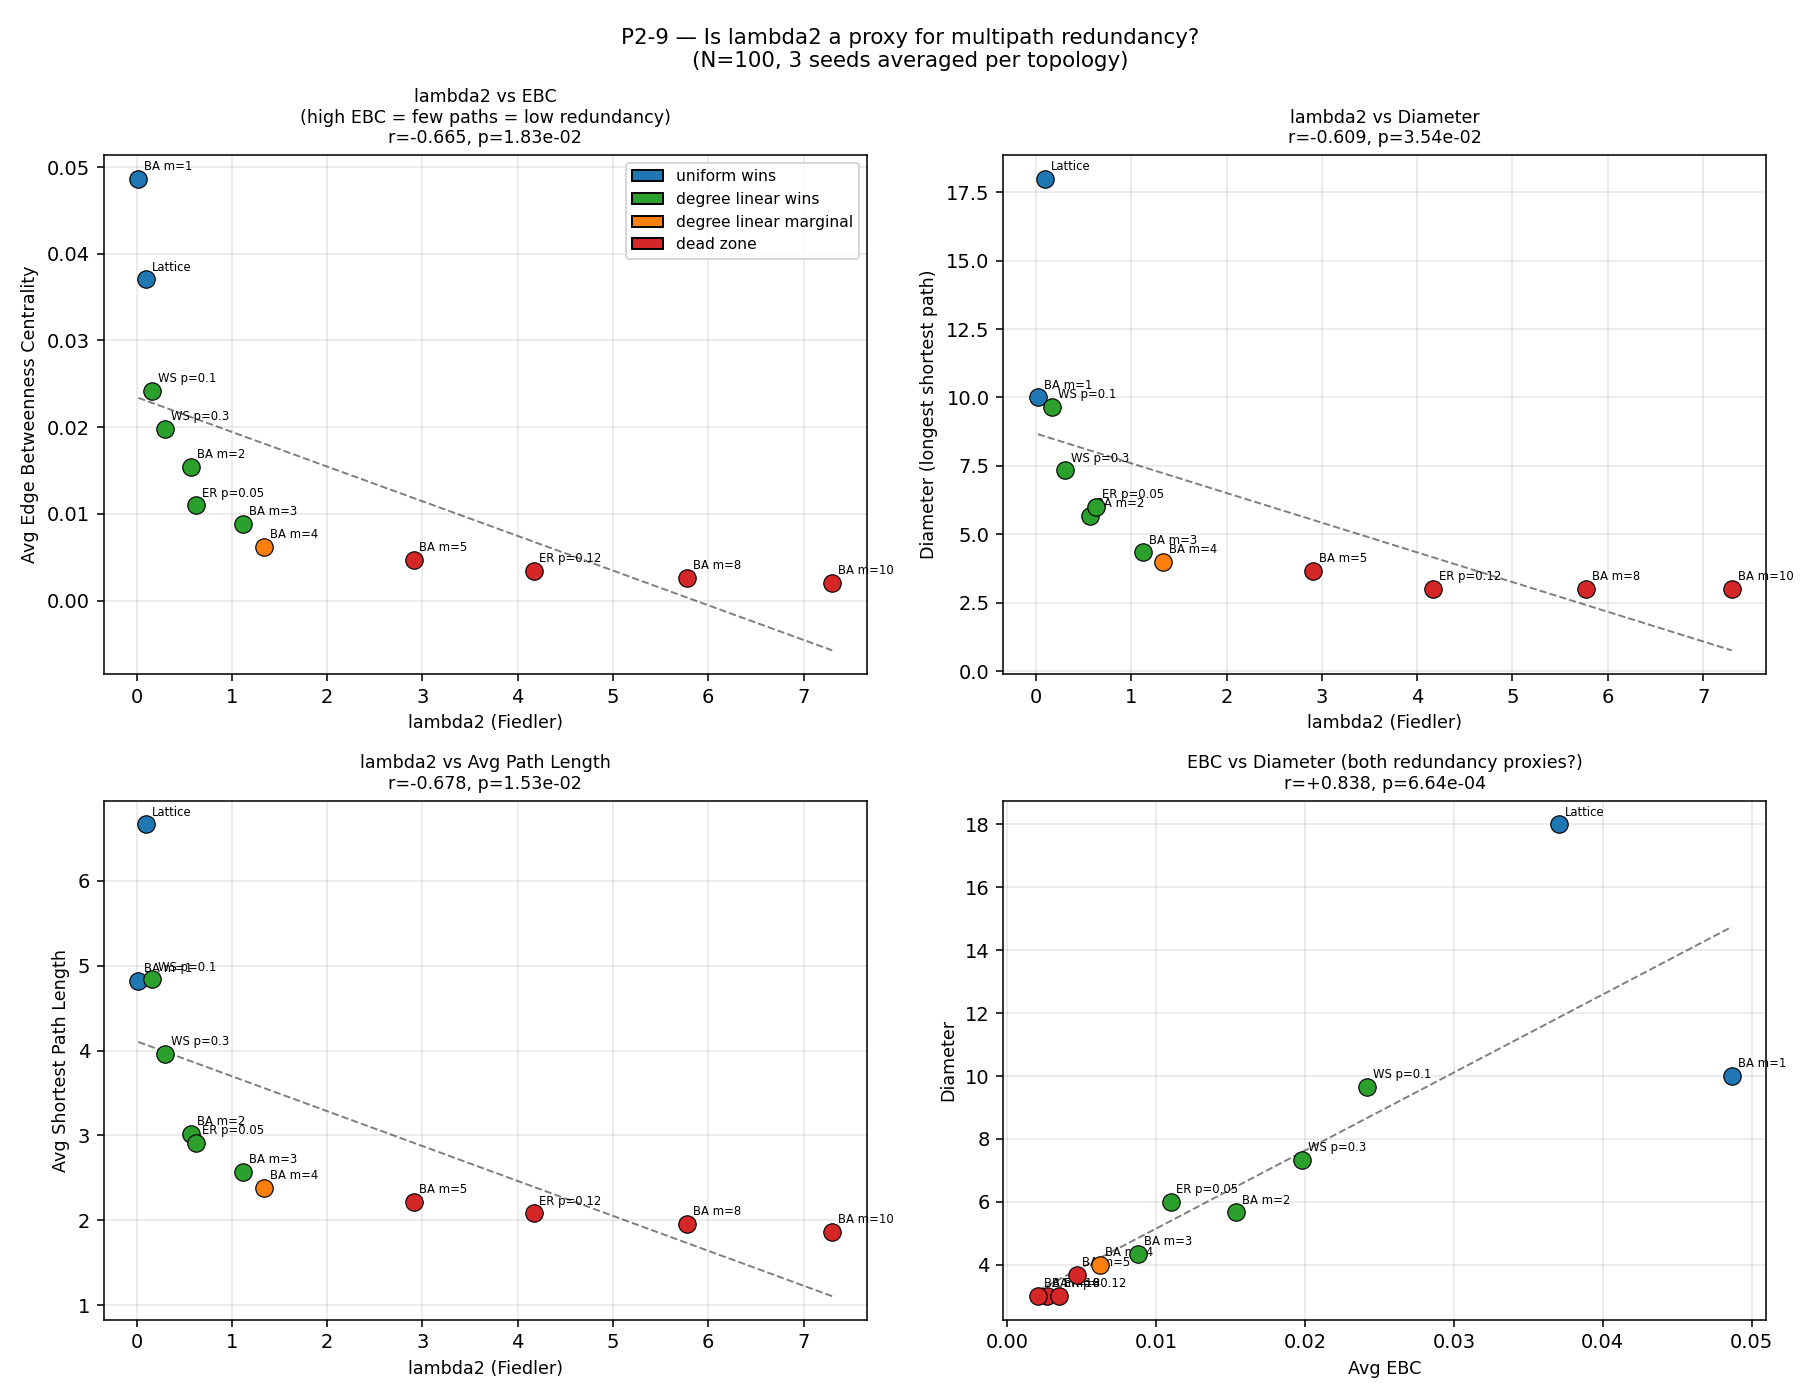
\includegraphics[width=\linewidth]{p2_edge_betweenness.png}
    \caption{Same metric plotted against edge betweenness centrality ($r = -0.604$), which fails to separate dead-zone topologies, confirming that $\lambda_2$ is the causal structural predictor.}
    \label{fig:edge_betweenness}
  \end{subfigure}
  \caption{Topological predictors of the dead zone. Algebraic connectivity $\lambda_2$ (Fiedler value) is a near-perfect predictor; edge betweenness is not.}
  \label{fig:topology_predictors}
\end{figure}

\begin{figure}[htbp]
  \centering
  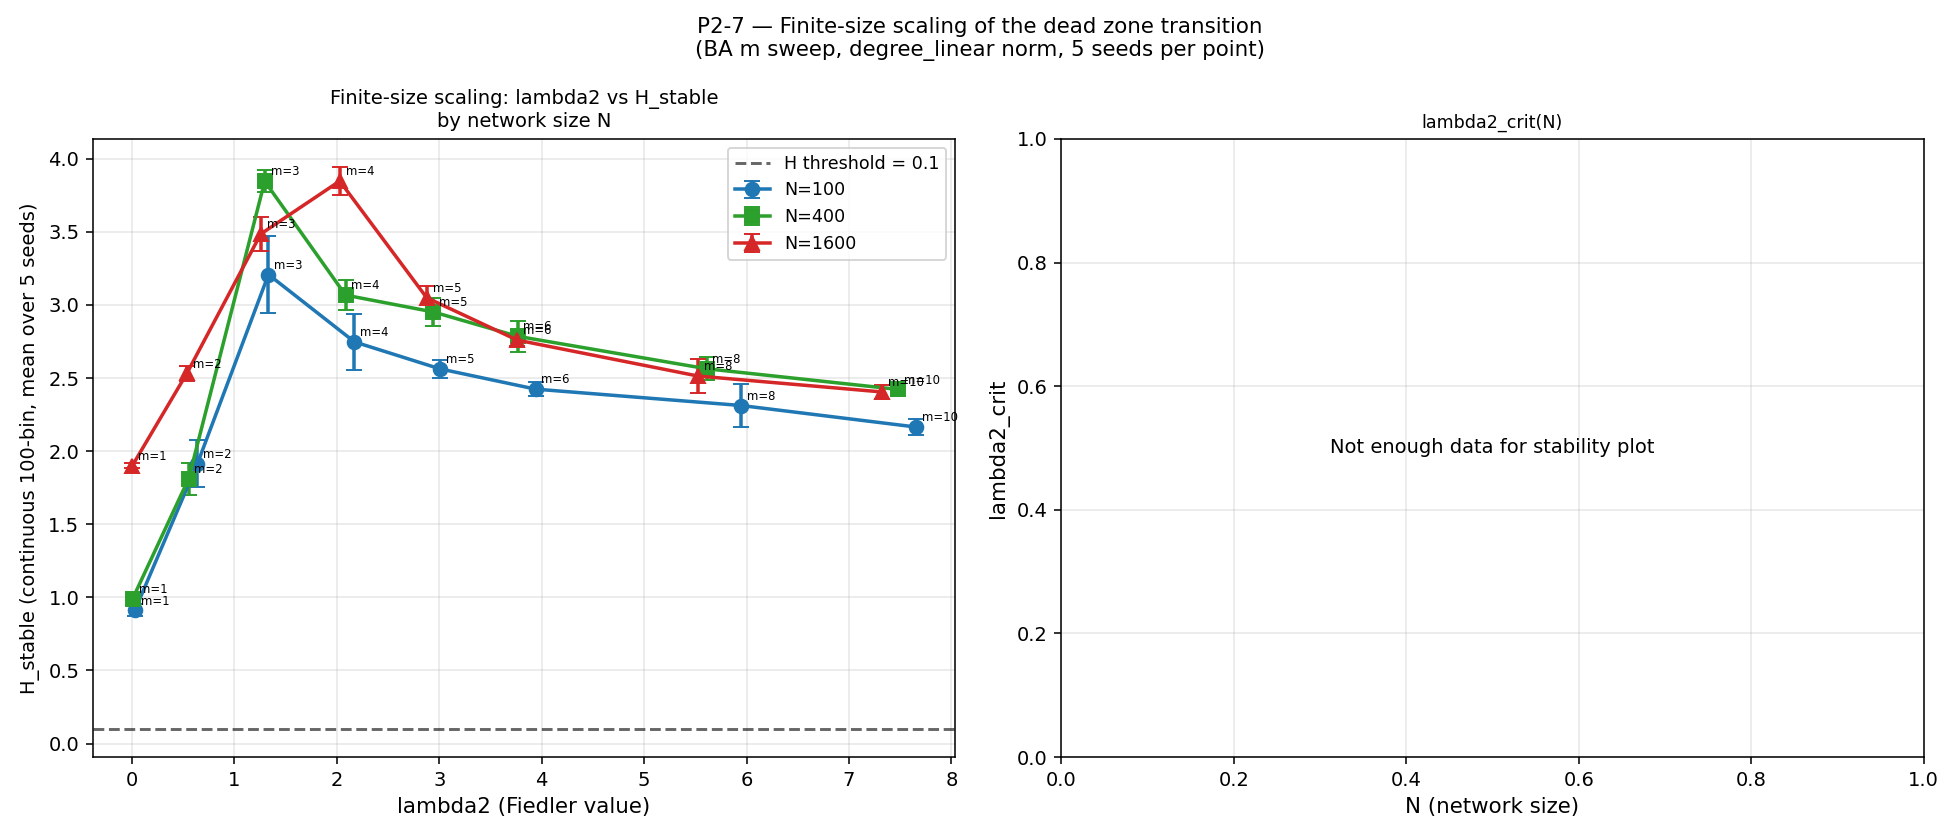
\includegraphics[width=0.88\linewidth]{p2_finite_size_scaling.png}
  \caption{Finite-size scaling of $\lambda_2$ and cognitive entropy for BA networks ($m=2,3,4,5$) from $N=100$ to $N=1600$. Fiedler values are nearly scale-invariant for a given $m$, confirming that $\lambda_{2,\mathrm{crit}} \approx 2.5$ is a structural property of the graph class, not an artifact of system size.}
  \label{fig:finite_size}
\end{figure}

Below $\lambda_{2,\mathrm{crit}}$, uniform digital Gaussian noise monotonically improves diversity via stochastic resonance. Above it, the path redundancy is so severe that no amplitude of Gaussian noise ($\sigma_v \le 1.20$) can fracture the synchronized manifold. Null results using directed noise strategies further confirm that the dead zone cannot be escaped through simple topological heuristics.

\begin{figure}[htbp]
  \centering
  \begin{subfigure}[b]{0.48\linewidth}
    \centering
    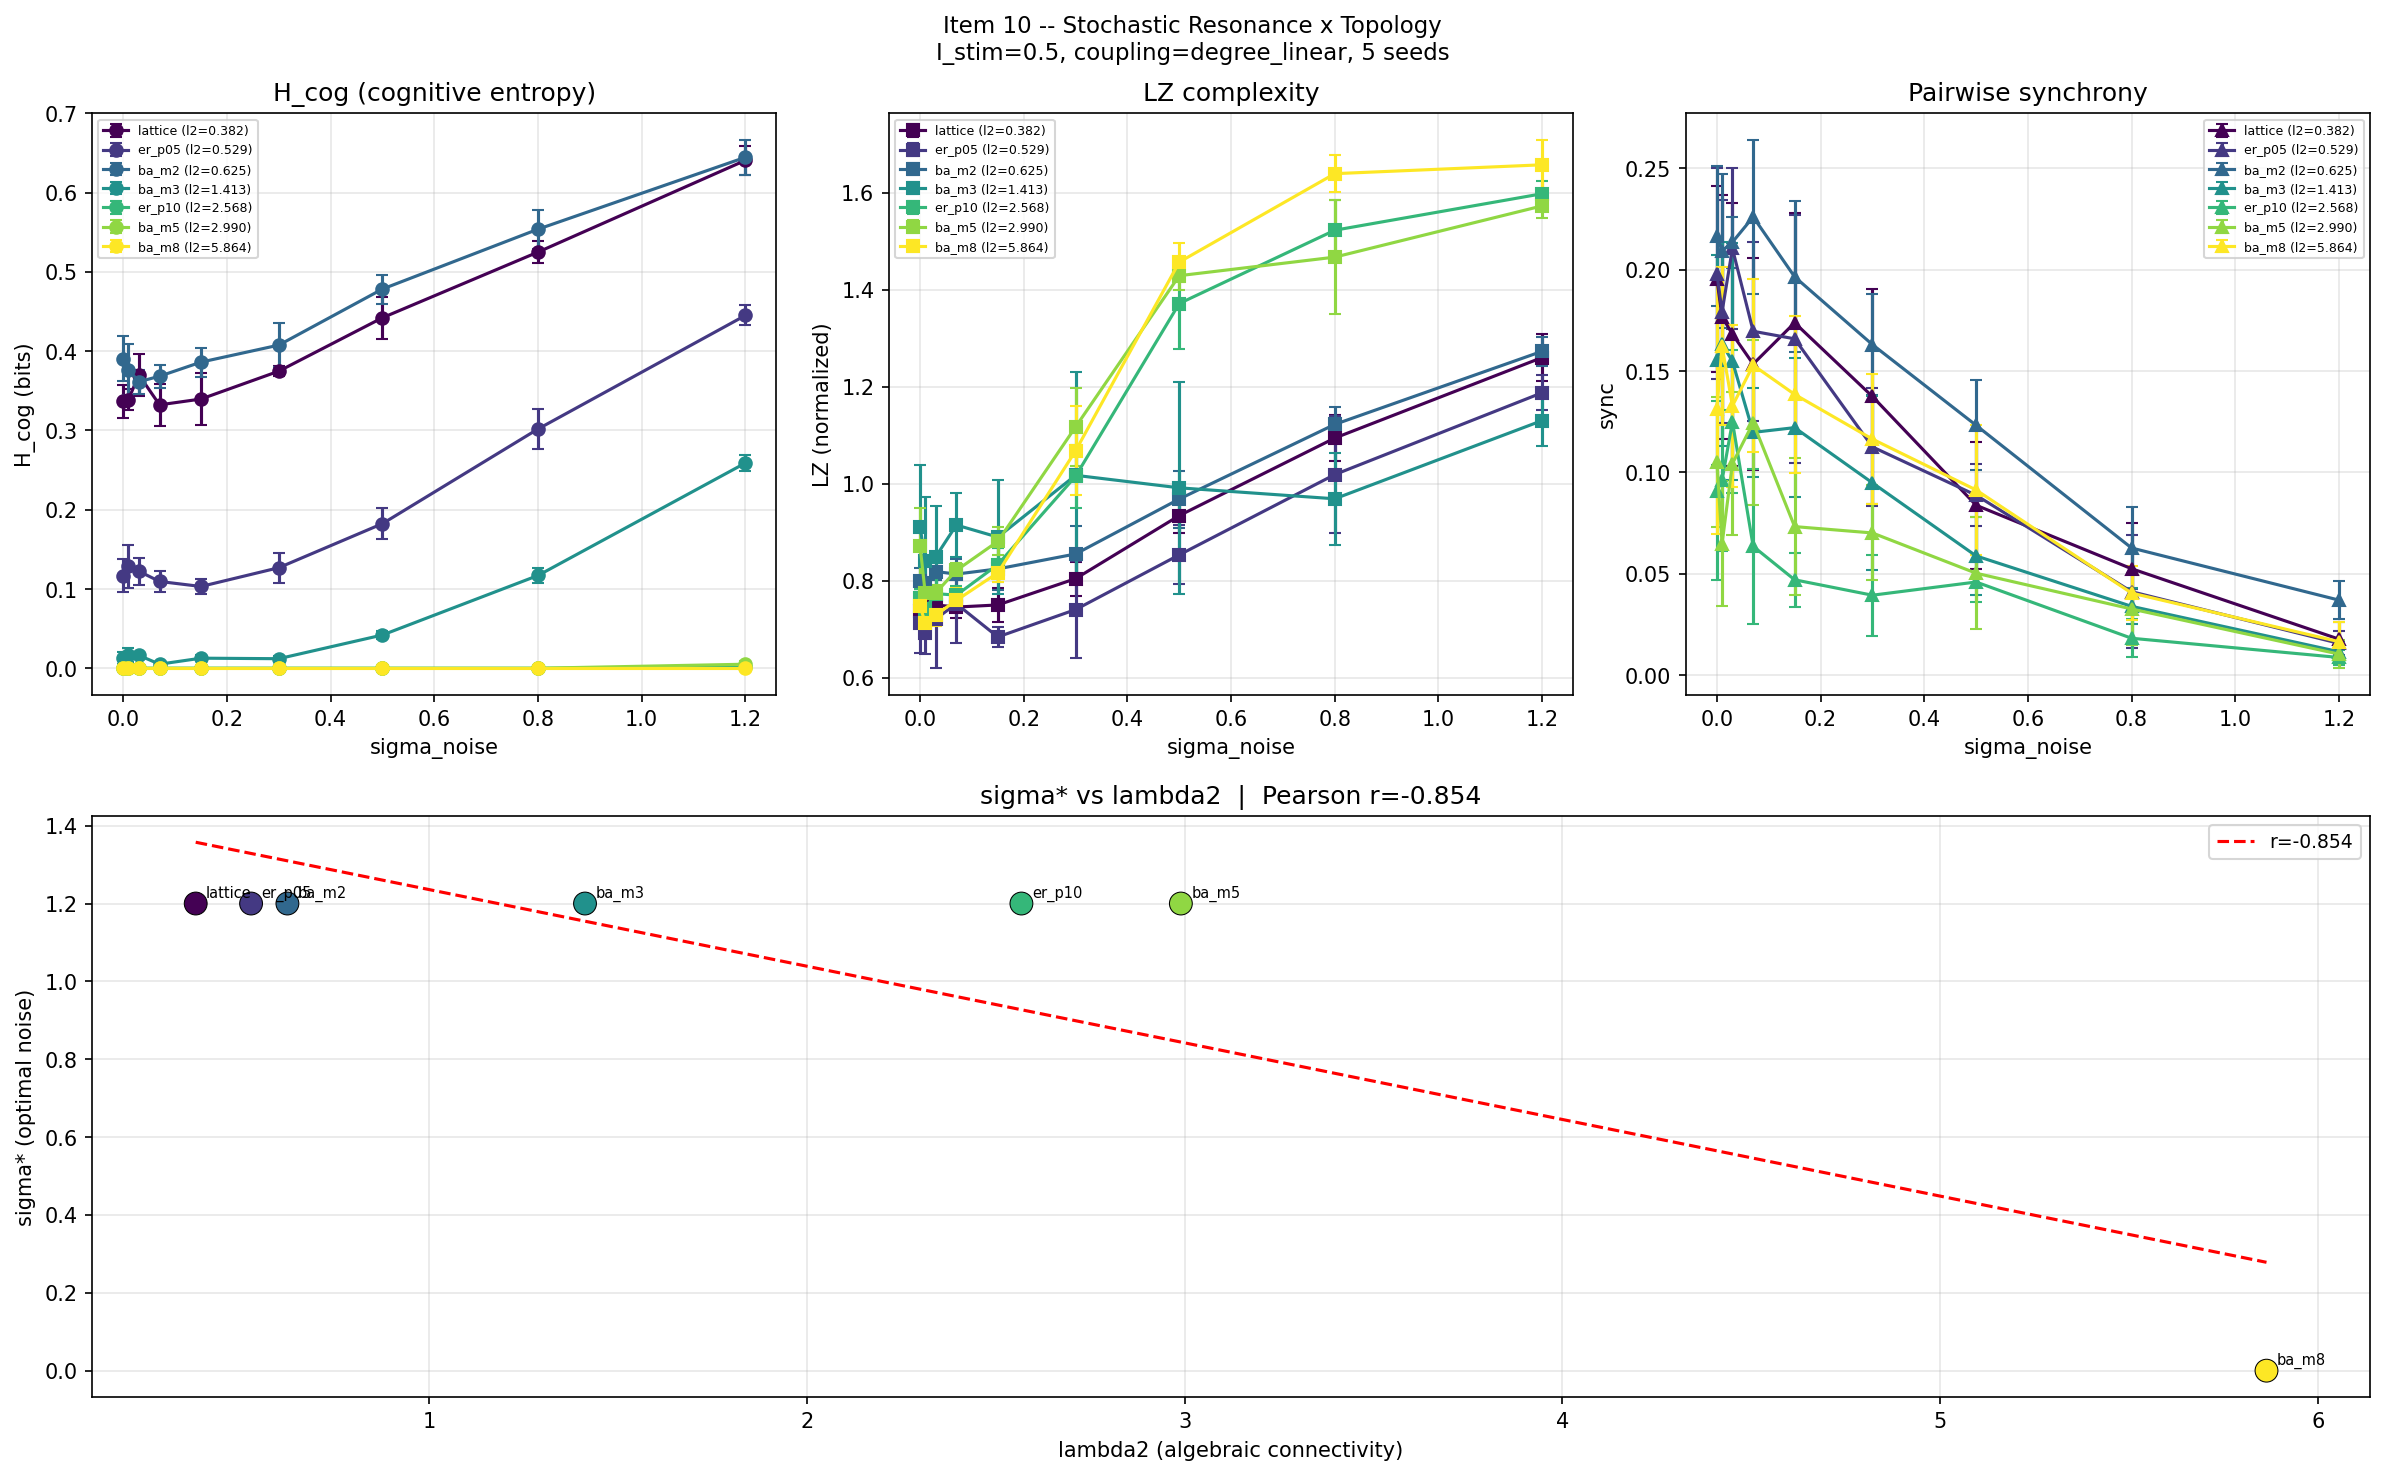
\includegraphics[width=\linewidth]{p2_stochastic_resonance_topology.png}
    \caption{Stochastic resonance landscape: $H_{\mathrm{cog}}$ vs.\ uniform noise amplitude $\sigma_v$ for four topologies spanning the $\lambda_2$ boundary. Topologies below $\lambda_{2,\mathrm{crit}}$ (Lattice, BA $m=2$) show monotonic improvement; those above (BA $m=5$) show no rescue at any tested $\sigma_v$.}
    \label{fig:sr_topology}
  \end{subfigure}
  \hfill
  \begin{subfigure}[b]{0.48\linewidth}
    \centering
    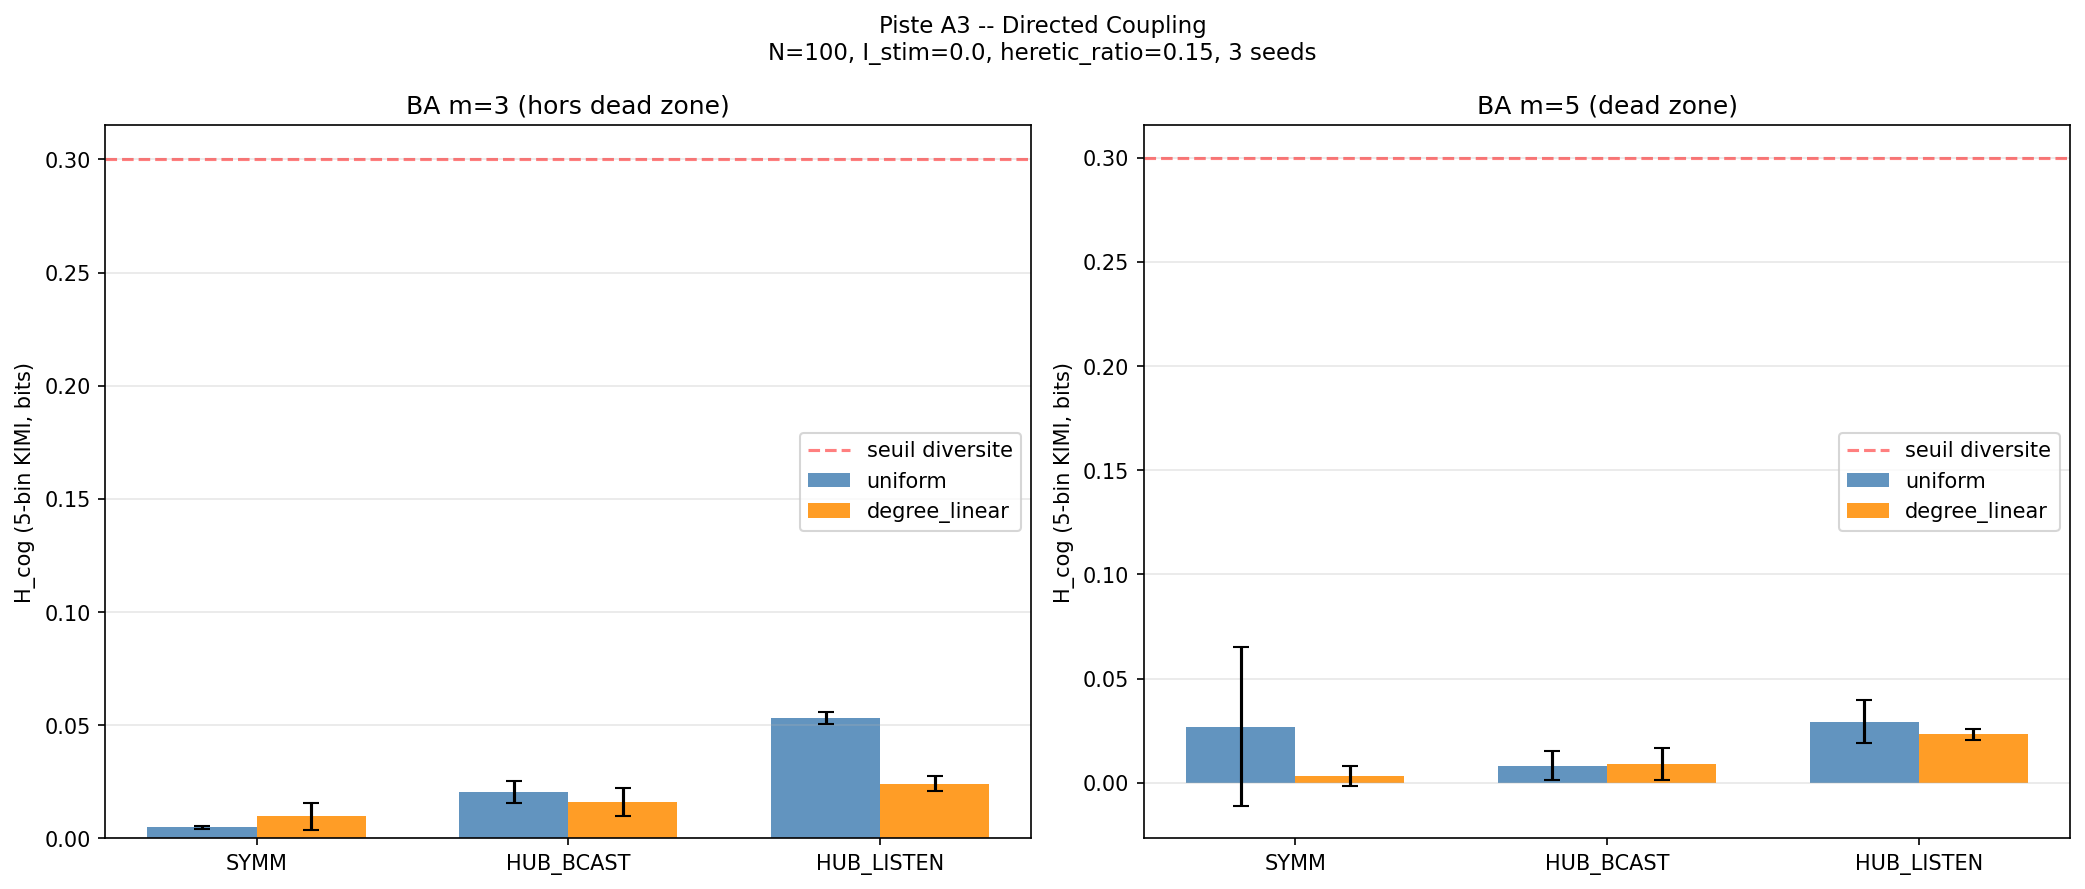
\includegraphics[width=\linewidth]{p2_directed_coupling.png}
    \caption{Null result: directed hub-targeted noise injection. Injecting noise selectively at high-degree nodes does not break synchrony in the dead zone (BA $m=5$), confirming that the barrier is a global spectral property, not a local hub effect.}
    \label{fig:directed_coupling}
  \end{subfigure}
  \caption{Stochastic resonance and null results for directed noise strategies. Neither uniform nor topologically targeted noise can rescue dead-zone topologies.}
  \label{fig:stochastic_resonance}
\end{figure}

\begin{figure}[htbp]
  \centering
  \begin{subfigure}[b]{0.48\linewidth}
    \centering
    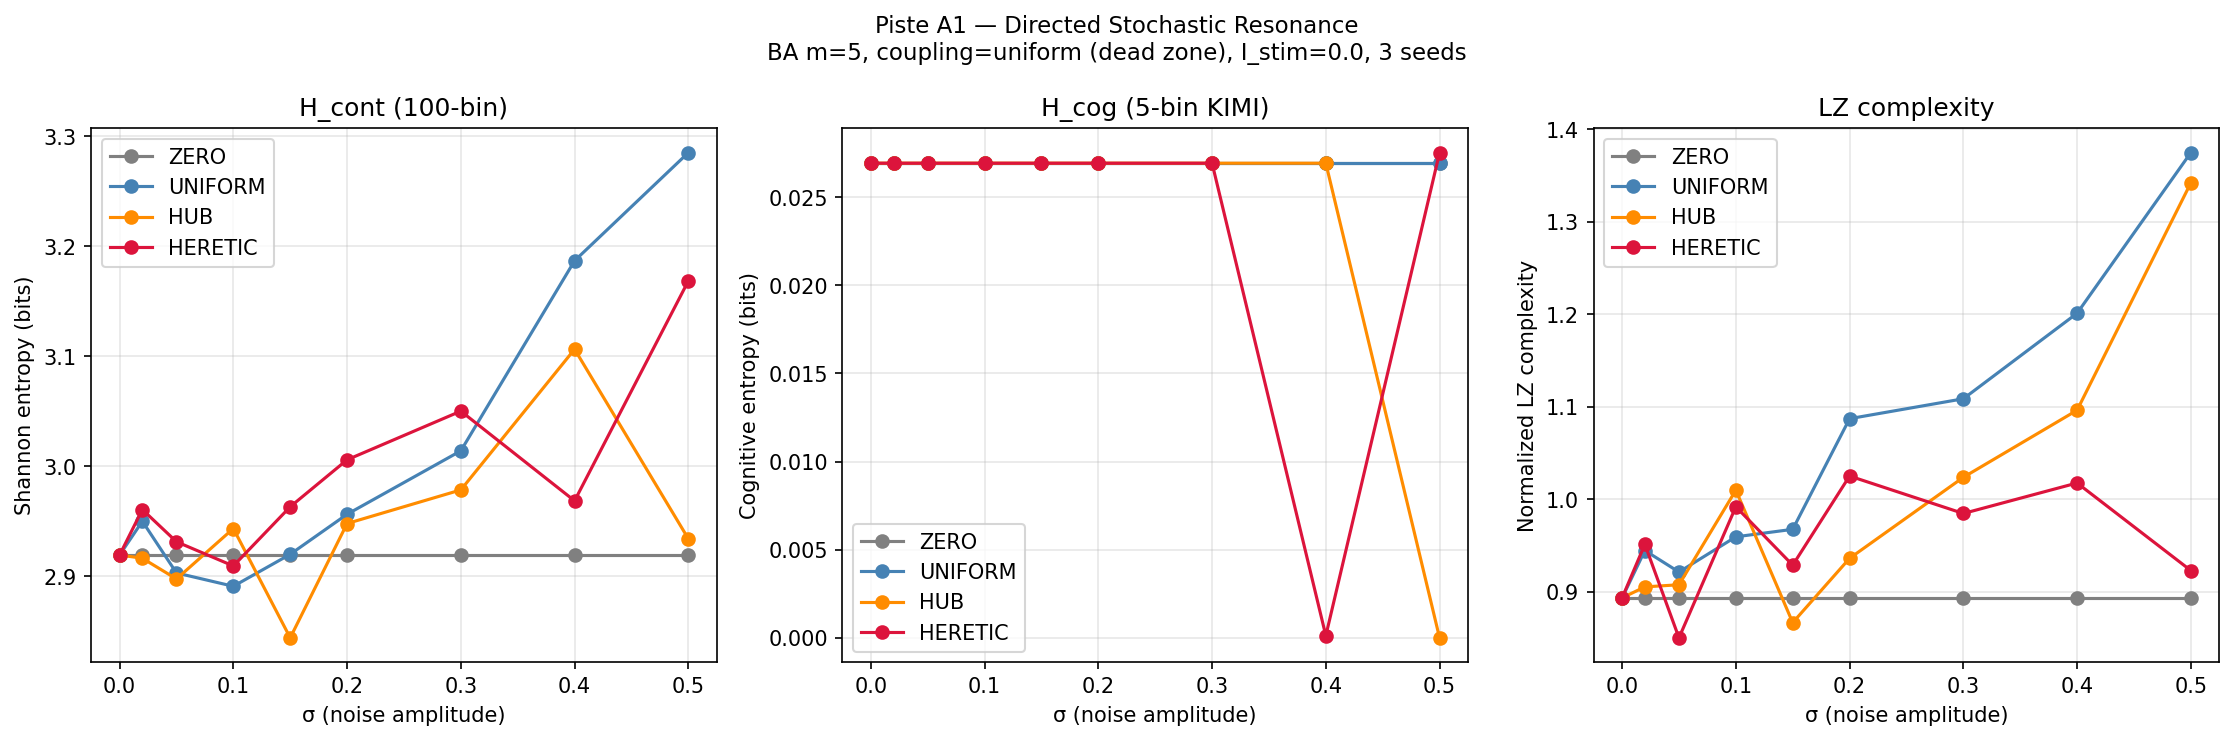
\includegraphics[width=\linewidth]{p2_stochastic_resonance_directed.png}
    \caption{Directed stochastic resonance (noise amplitude at hub vs.\ leaf nodes swept independently) on BA $m=5$. No combination rescues the dead zone.}
    \label{fig:sr_directed}
  \end{subfigure}
  \hfill
  \begin{subfigure}[b]{0.48\linewidth}
    \centering
    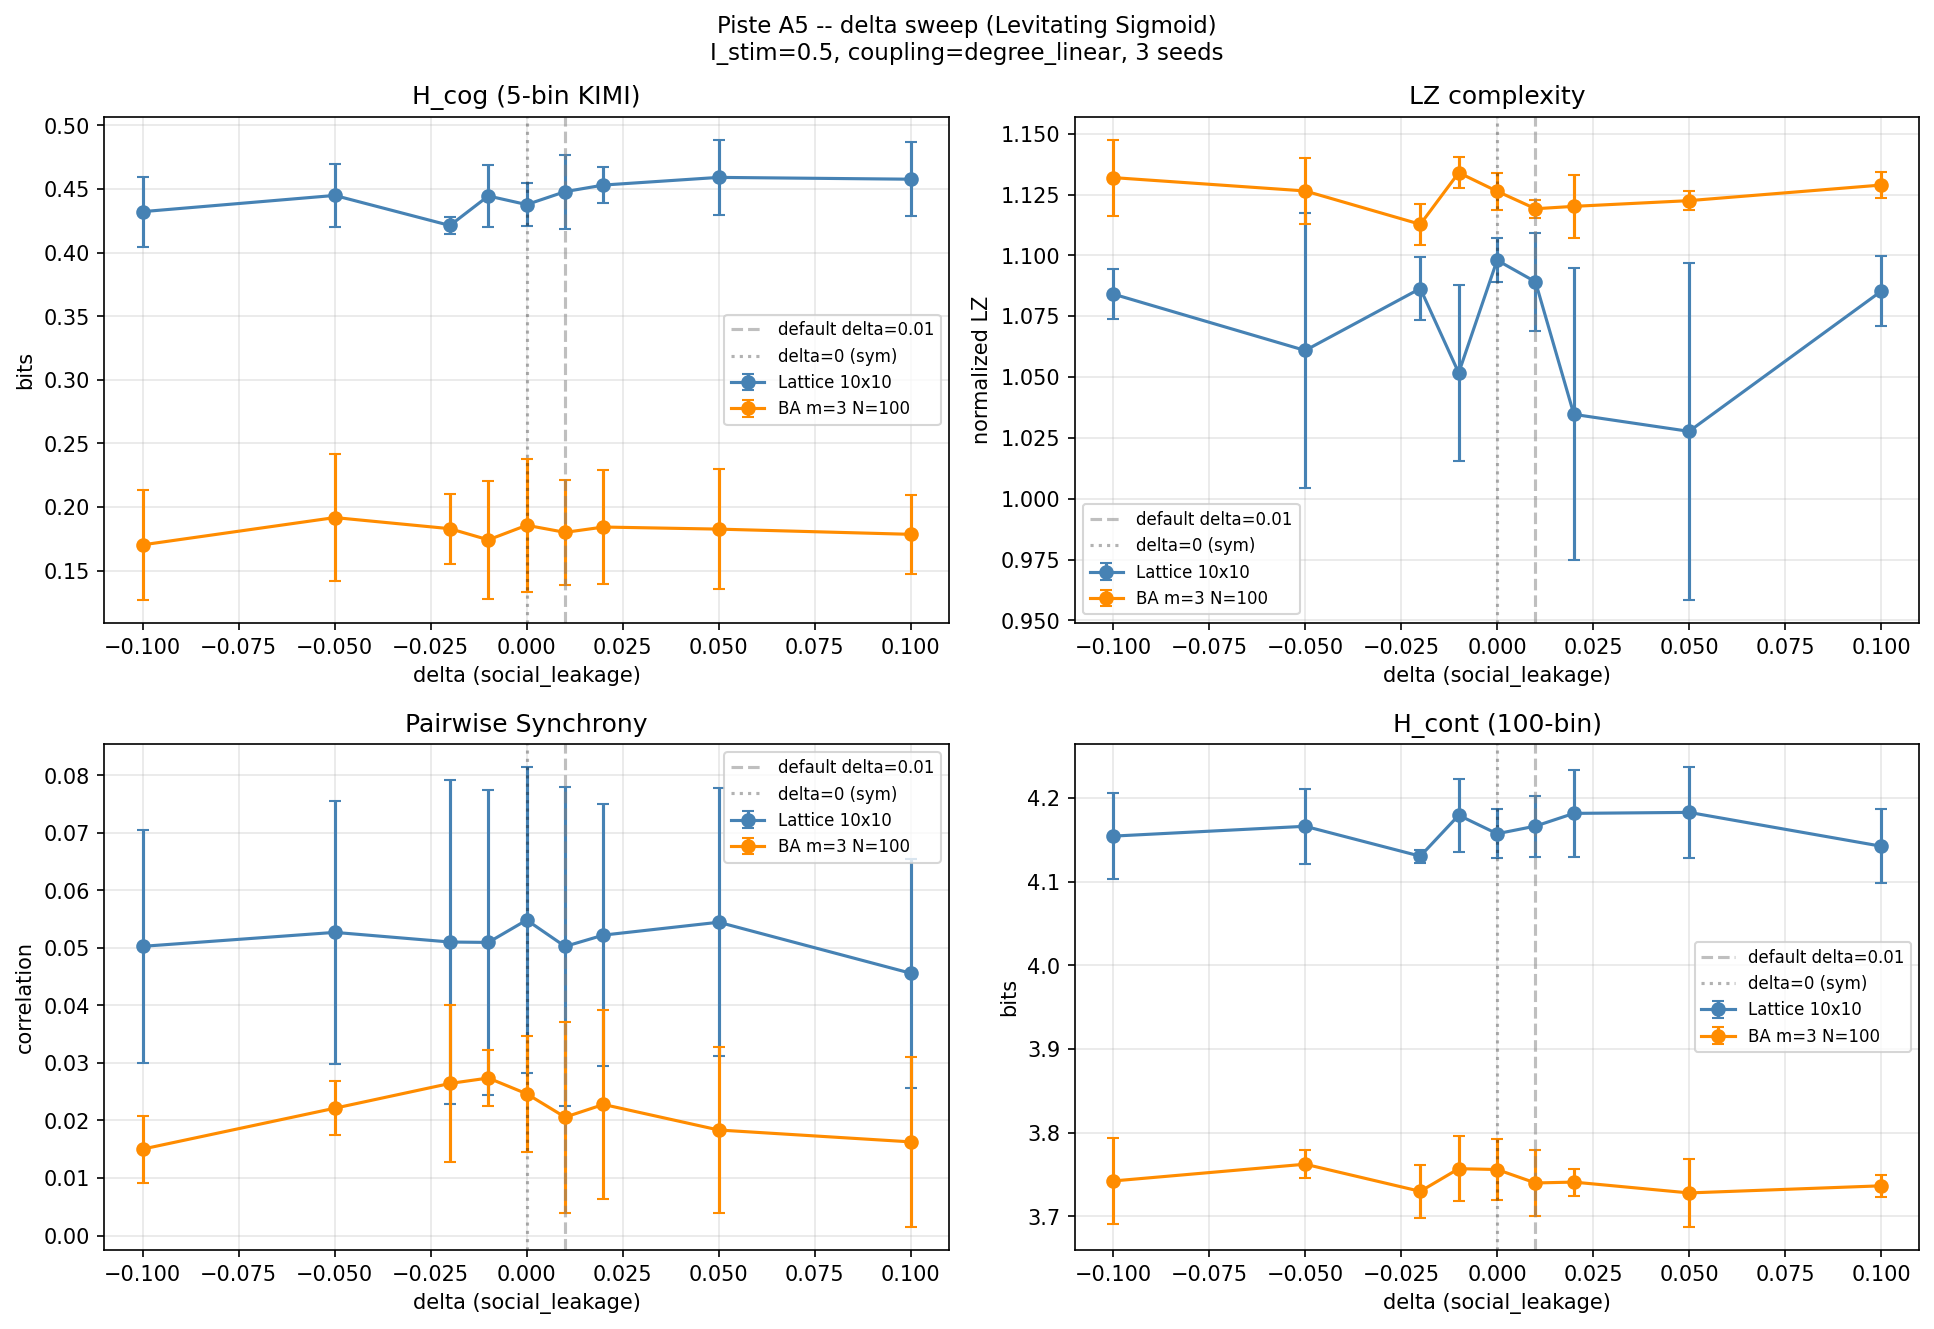
\includegraphics[width=\linewidth]{p2_delta_sweep.png}
    \caption{Sweep of the coupling asymmetry parameter $\delta$ (degree of directed coupling). Increasing $\delta$ does not lift $H_{\mathrm{cog}}$ in the dead zone, ruling out coupling-asymmetry rescue.}
    \label{fig:delta_sweep}
  \end{subfigure}
  \caption{Extended null results. Neither directed stochastic resonance nor coupling asymmetry ($\delta$-sweep) rescues dead-zone topologies.}
  \label{fig:null_results}
\end{figure}

\section{Doubt-Driven Community Structure}
\label{sec:communities}
We hypothesized that nodes experiencing synchronous fluctuations in their doubt variables form emergent functional communities that transcend the underlying physical topology. We constructed a doubt-affinity graph by thresholding the absolute Pearson correlation of the $u(t)$ traces and applied the Louvain method to extract doubt-driven communities.

While two distinct behavioral populations emerge---saturated singleton heretics ($u=1.0$) and large groups of collectively frustrated nodes---the alignment with structural communities is mixed. Using Normalized Mutual Information (NMI) against a rigorous bootstrap permutation baseline ($n=500$ permutations), the observed overlap is significant in 3 out of 6 tested seeds: regular-lattice seeds 42 and 123 ($z = +2.41$ and $z = +1.83$, $p < 0.05$) and BA $m=3$ seed 777 ($z = +2.55$, $p < 0.01$). The remaining three seeds show no significant overlap, and one BA seed exhibits anti-alignment ($z = -2.18$). The mean NMI across conditions is modest ($\overline{NMI} \approx 0.27$). We conclude that while doubt forms ``basins of collective frustration,'' these basins do not reliably decode the structural modularity of the network: the signal is topology- and seed-dependent, suggesting that emergent doubt communities reflect dynamical accidents rather than a principled structural readout.

\begin{figure}[htbp]
  \centering
  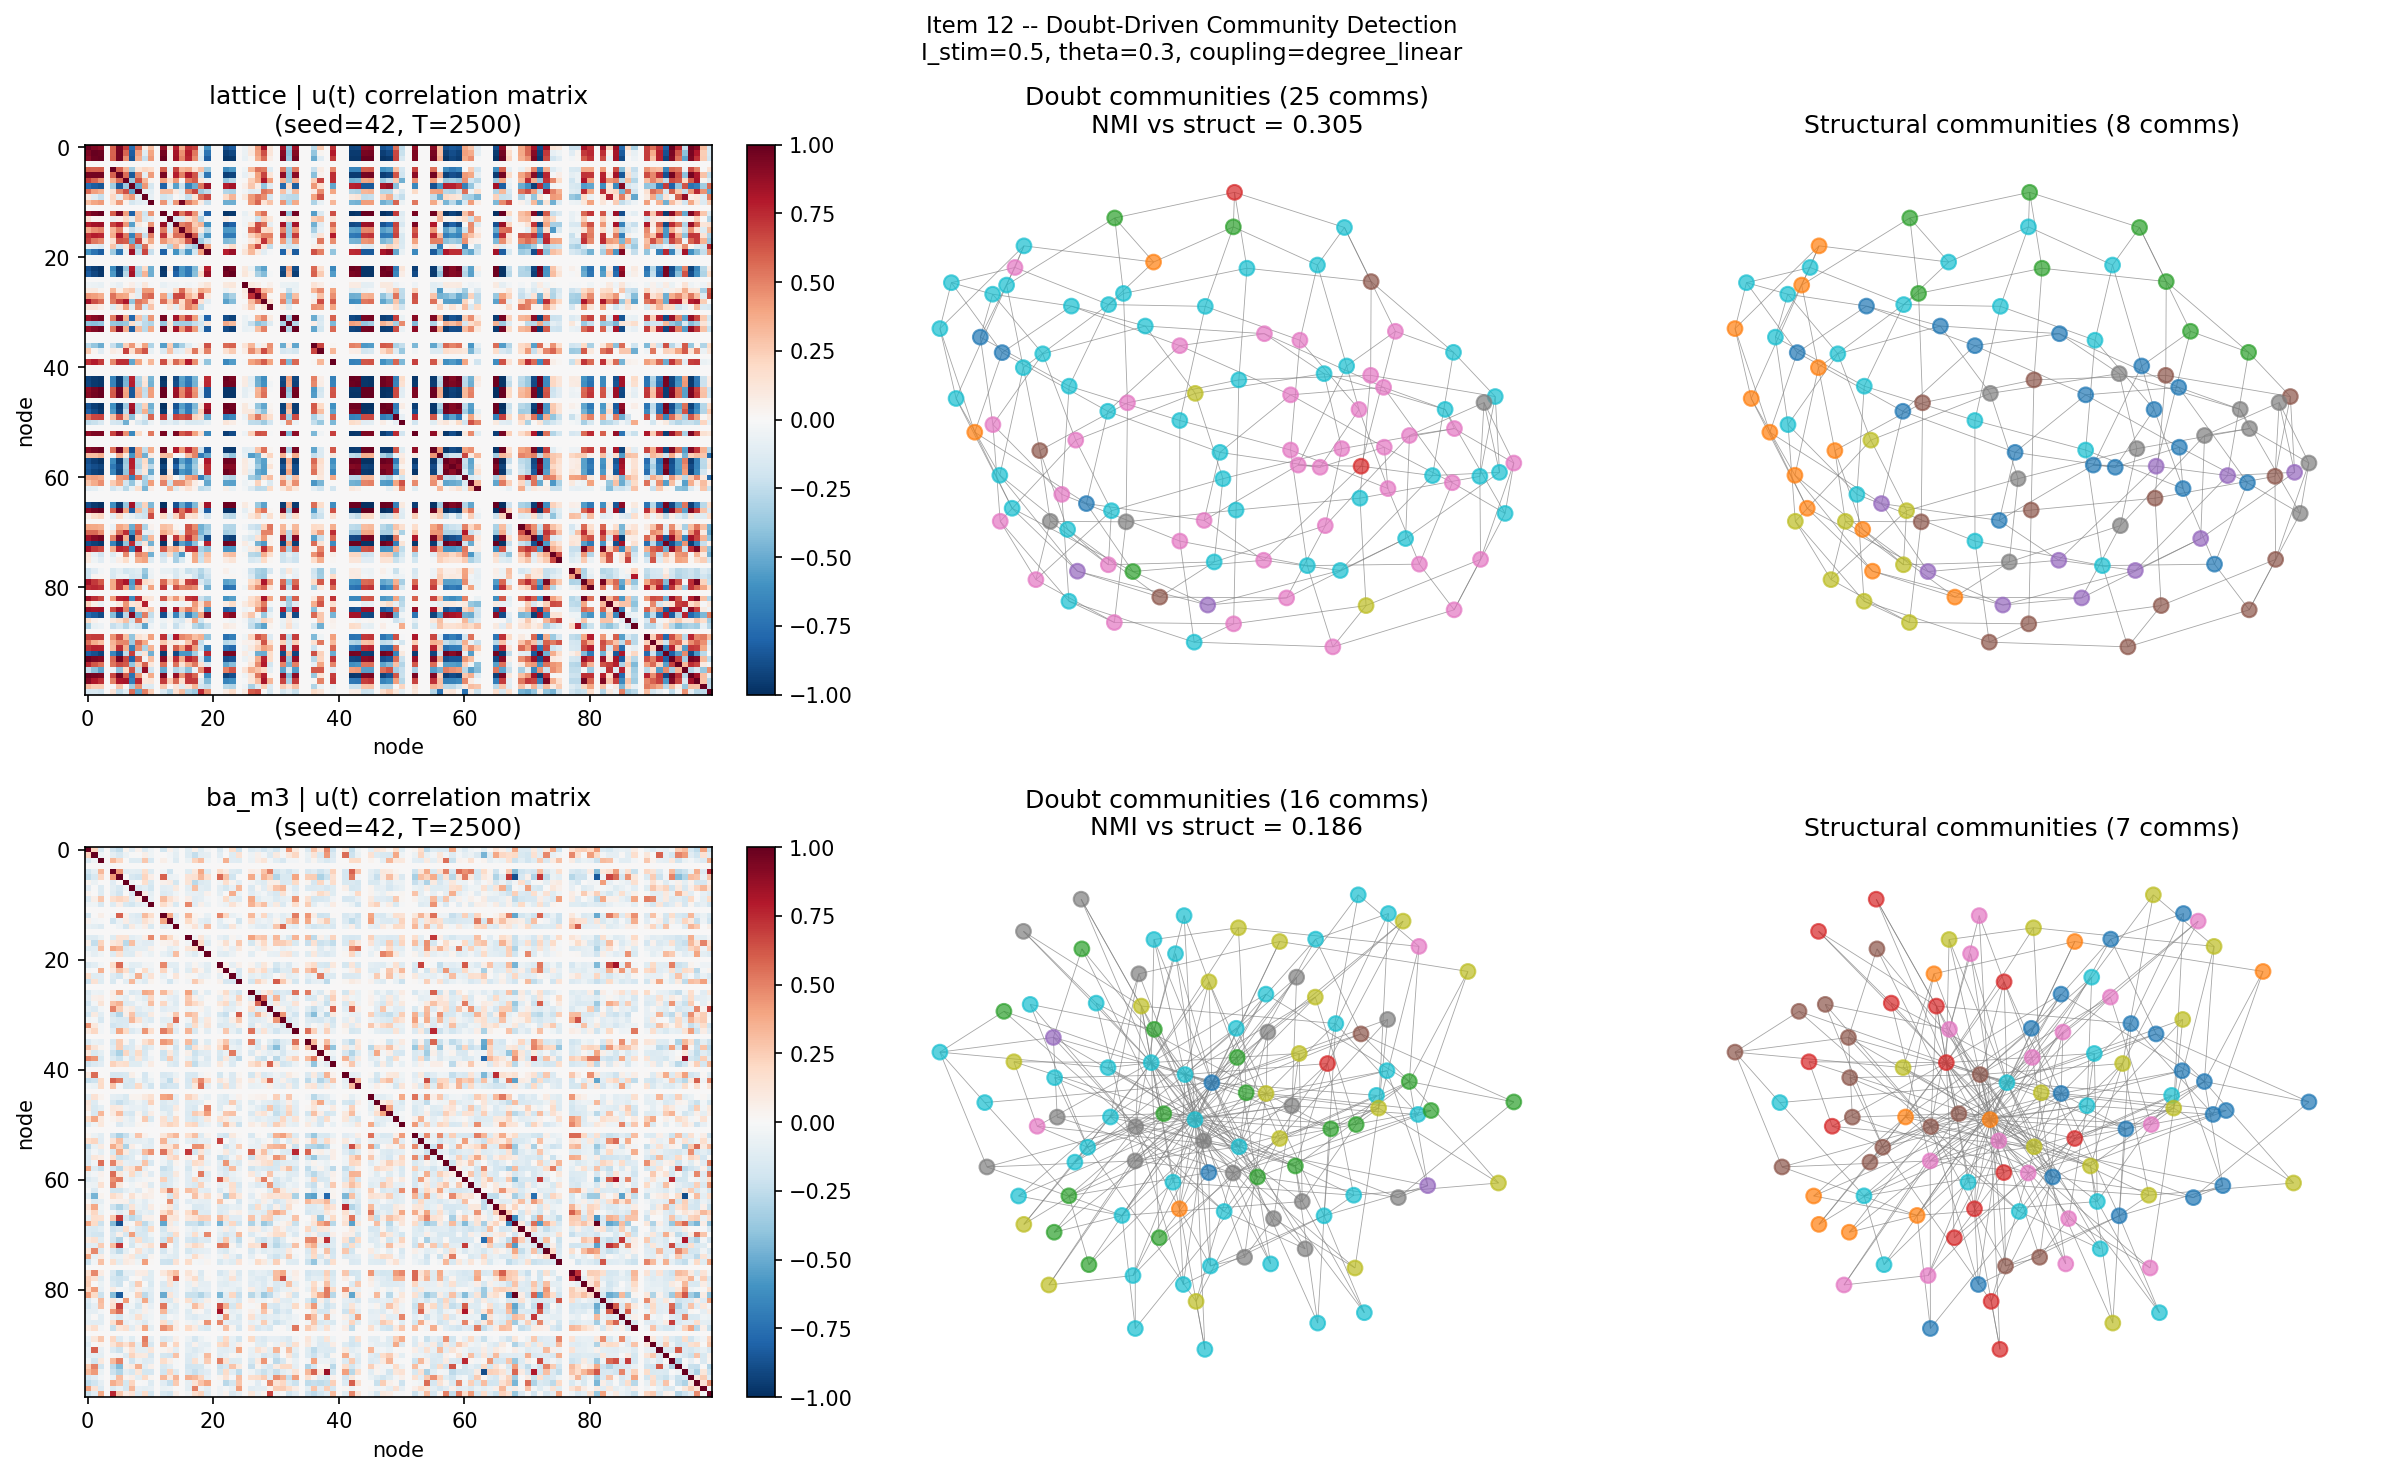
\includegraphics[width=0.88\linewidth]{p2_doubt_community_detection.png}
  \caption{Doubt-driven community detection results for regular lattice ($10{\times}10$) and BA $m=3$ ($N=100$), three seeds each. Left column: doubt-affinity graphs (edges coloured by Louvain community assignment). Right column: NMI $z$-score relative to 500 bootstrap-permuted baselines (horizontal dashed line: $z=1.96$). Filled bars indicate statistical significance ($p < 0.05$). Three of six seeds pass the threshold; results are inconsistent across topologies and seeds.}
  \label{fig:communities}
\end{figure}

\section{Discussion and Conclusion}
\label{sec:discussion}
The Mem4ristor architecture introduces a powerful mechanism for frustrated synchronization, but its limits are rigorously defined by the underlying graph topology. The doubt variable $u$ functions not as a passive decoder of local structure, but as a critical, adaptive anti-synchronization filter. Its timescale, $\tau_u$, acts as a master bifurcation parameter controlling the network's phase.

A limitation of the present study is that most experiments were averaged over $n=3$ independent seeds. The ablation (\S\ref{sec:mechanism}) and $\tau_u$ bifurcation (\S\ref{sec:bifurcation}) results have been replicated with $n=5$ seeds, confirming the reported effects; computationally intensive experiments (stochastic resonance topology sweep, finite-size scaling) remain at $n=3$ and are marked for extension before publication.

Crucially, the resilience of the topological dead zone above $\lambda_{2,\mathrm{crit}} \approx 2.5$ highlights a fundamental limitation of software-based, digitally integrated oscillator models. As explored in parallel hardware mappings (Paper B), the homogeneous Gaussian noise that fails to rescue the dead zone in software is qualitatively different from the heterogeneously correlated Johnson-Nyquist thermal noise inherent to analog substrates. The boundaries defined here therefore represent not just a mathematical phase transition, but the precise point at which physical analog computation becomes strictly necessary to unlock the full computational diversity of dense neuromorphic networks.

\end{document}
